%%%%%%%%%%%%%%%%%%%%%%%%%%%%%%%%%%%%%%%%%%%%%%%%%%%%%%%%%%%%%%%%%%%%%%
% Problem statement
\begin{statement}[
  problempoints=70,
  timelimit=1 sekunda,
  memorylimit=512 MiB,
]{Spiderman}

\setlength\intextsep{-0.1cm}
\begin{wrapfigure}[7]{r}{0.26\textwidth}
\centering
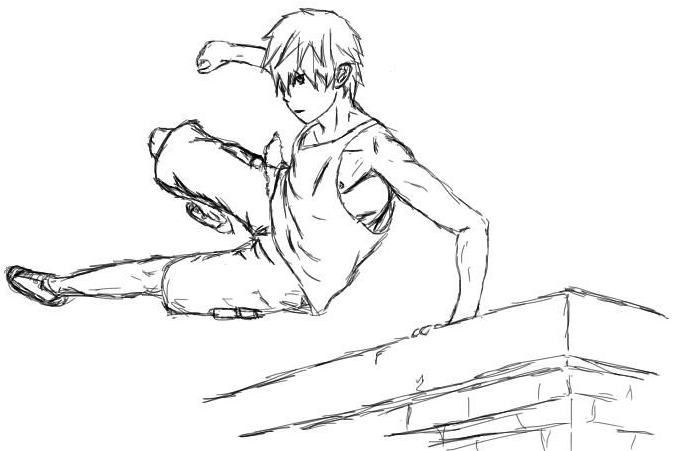
\includegraphics[width=0.26\textwidth]{img/spiderman.png}
\end{wrapfigure}

Mali Ivan veliki je obožavatelj društvene igre \textbf{Jamb} i Marvelovih
superjunaka.  Najdraži superjunak mu je čovjek-pauk, njujorški tinejdžer
prijateljima poznat kao Peter Parker koji je svoje supermoći stekao ugrizom
radioaktivnog pauka. Ivan mašta da će jednoga dana, baš kao čovjek-pauk,
slobodno vrijeme provoditi skačući s nebodera na neboder.  Usred jedne takve
maštarije, Ivan je usnuo.

U snu se više nije zvao Ivan, već Peter Parkour, singapurski tinejdžer koji
slobodno vrijeme provodi skačući s nebodera na neboder koristeći vještine
parkoura\footnote{Parkour -- metoda razvijanja ljudskog tijela kako bi bilo
sposobno kretati se što brže i efikasnije  kroz okolinu.}. Ivan, odnosno
Peter Parkour, zna da se u Singapuru nalazi točno $N$ nebodera te da je
$i$-ti neboder visok $h_i$ metara. Također, poznato mu je da zbog svojih
vještina može skočiti s $i$-tog na $j$-ti neboder ako je ostatak pri
dijeljenju $h_i$ s $h_j$ jednak $K$.  Pomozite Ivanu za svaki neboder
odrediti na koliko ostalih nebodera može s njega skočiti.

%%%%%%%%%%%%%%%%%%%%%%%%%%%%%%%%%%%%%%%%%%%%%%%%%%%%%%%%%%%%%%%%%%%%%%
% Input
\subsection*{Ulazni podaci}
U prvom su retku prirodan broj $N$ $(1 \le N \le 3\cdot10^5)$ i cijeli broj $K$
$(0 \le K < 10^6)$ iz teksta zadatka.

U sljedećem se retku nalazi $N$ prirodnih brojeva $h_i$ $(1 \le h_i \le 10^6)$
iz teksta zadatka.

%%%%%%%%%%%%%%%%%%%%%%%%%%%%%%%%%%%%%%%%%%%%%%%%%%%%%%%%%%%%%%%%%%%%%%
% Output
\subsection*{Izlazni podaci}
U jedinom retku ispišite $N$ cijelih brojeva tako da $i$-ti ispisani broj
odgovara broju nebodera na koje Peter Parkour može skočiti sa $i$-tog
nebodera iz ulaza.

%%%%%%%%%%%%%%%%%%%%%%%%%%%%%%%%%%%%%%%%%%%%%%%%%%%%%%%%%%%%%%%%%%%%%%
% Scoring
\subsection*{Bodovanje}
U testnim primjerima vrijednima $14$ bodova, vrijedit će $1 \le N \le 2\ 000$\\
U testnim primjerima vrijednima dodatnih $14$ bodova, postojat će najviše $2\ 000$
nebodera različitih visina.\\
U testnim primjerima vrijednima dodatnih $14$ bodova, vrijedit će $K = 0$.

%%%%%%%%%%%%%%%%%%%%%%%%%%%%%%%%%%%%%%%%%%%%%%%%%%%%%%%%%%%%%%%%%%%%%%
% Examples
\subsection*{Probni primjeri}
\begin{tabularx}{\textwidth}{X'X'X}
\sampleinputs{test/spiderman.dummy.in.1}{test/spiderman.dummy.out.1} &
\sampleinputs{test/spiderman.dummy.in.2}{test/spiderman.dummy.out.2} &
\sampleinputs{test/spiderman.dummy.in.3}{test/spiderman.dummy.out.3}
\end{tabularx}

\textbf{Pojašnjenje trećeg probnog primjera:}\\
S prvog nebodera visine $1$ Peter skočiti na bilo koji od preostalih nebodera.\\
S drugog nebodera visine $3$ Peter može skočiti samo na neboder visine $2$.\\
S trećeg nebodera visine $5$ Peter može skočiti samo na neboder visine $2$.\\
S četvrtog nebodera visine $7$ Peter može skočiti na neboder visine $2$ ili na neboder visine $3$.\\
S petog nebodera visine $2$ Peter ne može skočiti ni na koji od preostalih nebodera.

%%%%%%%%%%%%%%%%%%%%%%%%%%%%%%%%%%%%%%%%%%%%%%%%%%%%%%%%%%%%%%%%%%%%%%
% We're done
\end{statement}

%%% Local Variables:
%%% mode: latex
%%% mode: flyspell
%%% ispell-local-dictionary: "croatian"
%%% TeX-master: "../hio.tex"
%%% End:
